\documentclass[a4paper,12pt]{article}
\usepackage{indentfirst}
\usepackage[utf8]{inputenc}
\usepackage[english,russian]{babel}
\usepackage{listings}
\lstloadlanguages{[LaTeX] TeX, bash, Fortran, C++, make, Python}
\lstset{language =[LaTeX] TeX , extendedchars=true , escapechar =| ,frame=tb, commentstyle=\itshape, stringstyle =\bfseries}
\usepackage{graphicx,color}
\usepackage{subfigure}
\usepackage[centerlast,small]{caption2}
\usepackage{amsmath}
\usepackage{amssymb}
\usepackage[stable]{footmisc}
\usepackage{cite}
\sloppy
\oddsidemargin=5mm         %-левый отступ
\topmargin=-1cm             %-верхний отступ
\textwidth=16cm             %-ширина текста
\textheight=23cm            %-высота текста
\righthyphenmin=2           %-кол-во букв, разрешенных к переносу
 

\begin{document}

\begin{center}
\LARGE Численное моделирование трёхмерной упругой среды методом конечных элементов. 
\end{center}
	
	Перед тем, как читатель начнёт погружаться в изучение документации данной программы, ему следует сразу обратить на то, что представленная ниже программа никоим образом не может ставиться в один ряд с комплексами (коммерческими или свободно распространяемыми), которые на протяжении многих лет разрабатываются большими группами высококвалифицированных специалистов. Главной её целью является помощь начинающему разработчику или программисту в формировании представлений о разработке численных кодов, которые на одну ступень выше, чем на базовых уроках по численным методам в технических ВУЗах. 
  	
	%Представленная ниже программа была разработана исключительно в учебно-исследовательских целях, чтобы  не пришлось тратить время на множество проб и ошибок. %, совершённых  автором при реализации своих проектов.   
	
	Программа написана на языке C++ с использованием стандартной библиотеки (STL) без каких-либо иных сторонних библиотек. Так как изначально в разработке программы был сделан упор на создание расчётного ядра, как центрального элемента любого вычислительного комплекса, создание расчётных сеток и визуализация полученных результатов делегируется комплексам Gmsh и Paraview.

	От читателя требуется иметь базовое понимание метода конечных элементов (Зинкевича, Сегерлида, Павленко), языка программирования C++ и элементарных навыков работы с комплексами Gmsh и Paraview (будет в кратце описано).  

\section{Структура программы.}
	
	Программа разбита на несколько файлов о структуре которых будет рассказано ниже.

\begin{small}
\begin{verbatim}	
input.inp - входной файл. Имеется возможность здания как точечного силового 
            воздействия, так и нагружения на выбранной границе.
    mesh/ - папка с входным файлом \*.geo для сеткопостроителя GMSH и файлом 
            построенной сетки \*.mesh.
 results/ - папка с результатами.
src/..
   object.h - массивы классов узлов, граничных и поверхностных (ячеек) элементов.
   numerical.h - численные параметры (масштабирование сетки).
src/paraview/..
            out.cpp - генерация выходного файла для визуализатора Paraview.          
src/reader/..
          read_input_file.cpp - чтение входного файл input.inp. 
          construction_mesh.cpp - построение связей между элементами (узлами, элементами).
src/solver/..
   boundary.cpp - установка неподвижных граничных условий.
   geometry.cpp - вычисление объёма и матрицы Коши для элементов [1].
   linalg.cpp - вычисление СЛАУ методом сопряжённых градиентов [2].
   shift.cpp -  определение матрицы Гука, расчёт матриц локальной и глобальной жёсткости.
   solver.cpp - файл поэтапного вызова главных расчётных функций.
   stress_value.cpp - вычисление тензоров деформаций и напряжений для каждого элемента.
\end{verbatim}
\end{small}  
	
\section{Общая информация о методе конечных элементов.}
	
   	Здесь мы не будем вдаваться в глубокие математические подробности обоснования метода конечных элементов, читатель может легко найти информацию в широкой массе учебников. В данной документации приведём лишь общую информацию. Более детальную информацию автор советует смотреть в Зинкевича и Сегерлида.
   	
	Обратный закон Гука в матричной форме для среды в напряжённом состоянии можно записать следующим образом:
	\begin{equation}
	\sigma = A \epsilon
	\end{equation}
	где A - матрица упругости, $\epsilon$ - тензор деформаций, $\sigma$ - тензор напряжений.	
	
	В развёрнутом система уравнений может быть записана следующим образом:
\begin{equation}
\begin{Bmatrix}
 \sigma_{xx} \\
 \sigma_{yy} \\
 \sigma_{zz} \\ 
 \tau_{xy}   \\
 \tau_{yz}   \\
 \tau_{zx}    
\end{Bmatrix}
= \frac{E(1-\nu)}{(1+\nu)(1-2\nu)}
\begin{Bmatrix}
 1 & \frac{\nu }{1-\nu} & \frac{\nu }{1-\nu} & 0 & 0 & 0 \\
 \frac{\nu }{1-\nu} & 1 & \frac{\nu }{1-\nu} & 0 & 0 & 0 \\
 \frac{\nu }{1-\nu} & \frac{\nu }{1-\nu} & 1 & 0 & 0 & 0 \\
 0 & 0 & 0 & \frac{1-2\nu}{2(1-\nu)} & 0 & 0 \\ 
 0 & 0 & 0 & 0 & \frac{1-2\nu}{2(1-\nu)} & 0 \\ 
 0 & 0 & 0 & 0 & 0 & \frac{1-2\nu}{2(1-\nu)} \\       
\end{Bmatrix}
\begin{Bmatrix}
\frac{\partial u}{\partial x} \\
\frac{\partial v}{\partial y} \\
\frac{\partial w}{\partial z} \\
\frac{\partial u}{\partial y}+\frac{\partial v}{\partial x} \\
\frac{\partial v}{\partial z}+\frac{\partial w}{\partial y} \\
\frac{\partial w}{\partial x}+\frac{\partial u}{\partial z} \\
\end{Bmatrix}
\end{equation}
где x,y,z - координаты узлов, u,v,w - перемещения.

Предполагается, что модуль Юнга $E$ и коэффициент Пуассона $\nu$ для исследуемого материала известны. 

Сборка глобальной матрицы жёсткости и решение получившейся системы линейных алгебраических уравнений. При успешном разрешении системы будут получены итоговые перемещения узлов расчётной сетки, далее для каждого элемента вычисляются деформации и напряжения.

Система линейных алгебраических уравнений представлена ниже:
\begin{equation}
(V\: B^T\cdot A\cdot B) \vec{U} = F
\end{equation}
где $(V\: B^T\cdot A\cdot B)$ - есть глобальная матрица жёсткости, $\vec{U}$ - вектор перемещений.

Составление и решение данной СЛАУ является самым трудоёмким этапом, после которого вычисление деформаций и напряжений для каждого элемента не представляет каких-либо сложностей.


	При создании программы фундаментальным предположением было следующее: элемент есть объект, в котором могут быть заданы любые интересующие нас свойства. 

	В данном случае объектами являются узел, сегмент и ячейка.

	(рисунок)
 	
\section{Логика реализации.}   
	Ниже представлено поэтапное решение задачи методом конечных элементов с указанием файлов, где эти операции выполняются. 

\begin{itemize}
 		\item[•] Этап 1. Инициализация
 	\begin{itemize}
 		\item[1.] Чтение входного файла ($read\_input\_file.cpp$).
 		\item[2.] Определение связей между элементами сетки ($construction\_mesh.cpp$).
 		\item[3.] Определение всех параметров ($read\_input\_file.cpp$).		 		
	\end{itemize} 		 			
 		
 		\item[•] Этап 2. Решение
 	\begin{itemize}
 		\item[1.] Вычисление объёмов элементов ($geometry.cpp$).		
 		\item[2.] Вычисление матрицы $B$ для каждого элемента ($geometry.cpp$).	
 		\item[3.] Вычисление матрицы обратной матрицы $B^T$ для каждого элемента ($shift.cpp$).	
 		\item[4.] Определение матрицы упругости для каждого элемента ($shift.cpp$).	
 		\item[5.] Определение локальных матриц для всех элементов ($shift.cpp$).	 				 		
 		\item[6.] Сборка локальных матриц в глобальную матрицы жёсткости ($shift.cpp$).	 
 		\item[7.] Определение граничных условий ($boundary.cpp$).	 
 		\item[8.] Модификация глобальной матрицы согласно граничным условиям ($linlag.cpp$).	   		 				 				 		
 		\item[9.] Подстановка нагрузок ($linlag.cpp$).	 		
 		\item[10.] Расчёт СЛАУ методом сопряжённых градиентов ($linlag.cpp$).	  		 				 				 		 		
 		\item[11.] Вычисление тензора деформаций ($stress\_value.cpp$).	
 		\item[12.] Вычисление тензора напряжений ($stress\_value.cpp$).			 		
	\end{itemize} 		
	
 		\item[•] Этап 3. Вывод
 	\begin{itemize}
 		\item[1.] Запись полученных результатов ($out.cpp$).		
	\end{itemize} 		
\end{itemize}	
		

\section{Этапы.} 

 	\subsection{Этап 0.}
 	
 	Прежде чем приступить к рассмотрению структуры программы следует разобраться в принципе построения расчётной сетки. Как было указано выше разработка программы-сеткопостроителя является отдельной задачей, рассмотрение которой выходит за рамки настоящего руководства. В качестве решения задачи с построением сетки был выбран свободно распространяемый и достаточно функциональный комплекс Gmsh [], в котором за достаточно короткое время можно научиться строить неструктурированные сетки, в том числе и со сложной геометрией.
 	
\begin{figure}
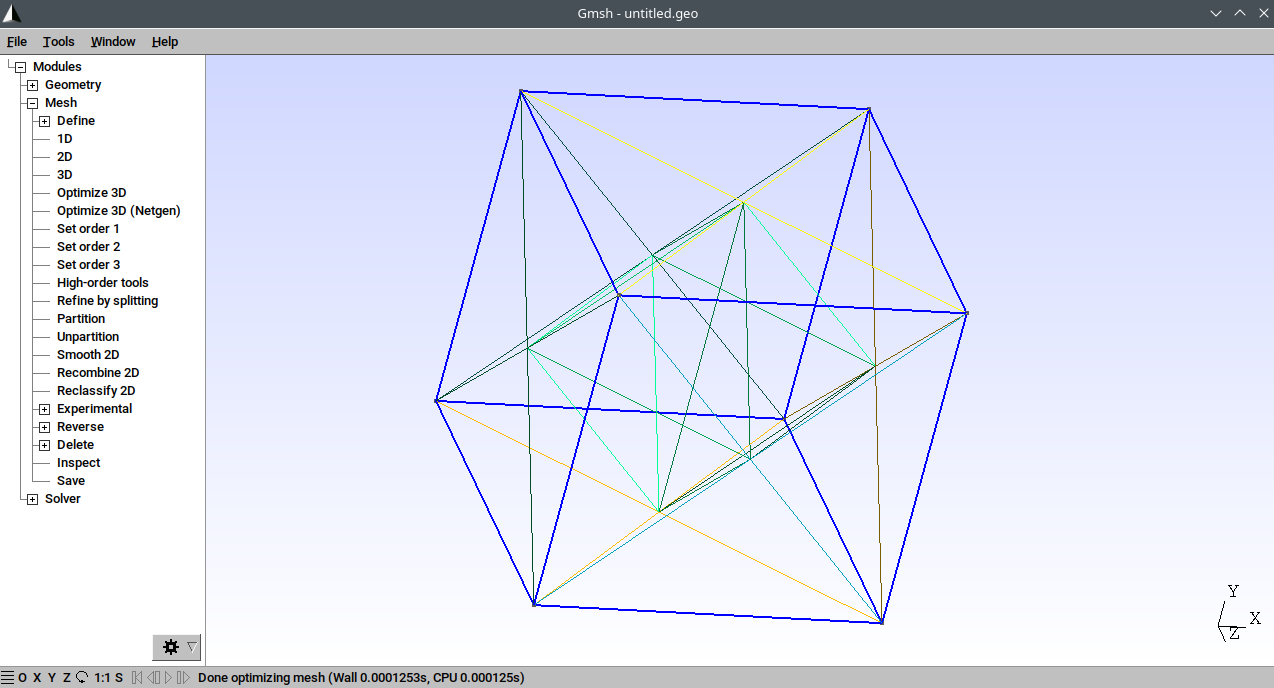
\includegraphics[scale=0.5]{gmsh.png}
\caption{•}
\end{figure} 	

В качестве примера ниже представлен GMSH-файл для генерации неструктурированной трёхмерной сетки, ячейками которой являются тетраэдры.
\begin{small}
\begin{verbatim}	
//+
Point(1) = {0, 0, 0, 1.0};
//+
Point(2) = {0, 1, 0, 1.0};
//+
Point(3) = {0, 1, 1, 1.0};
//+
Point(4) = {0, 0, 1, 1.0};
//+
Point(5) = {1, 0, 0, 1.0};
//+
Point(6) = {1, 1, 0, 1.0};
//+
Point(7) = {1, 1, 1, 1.0};
//+
Point(8) = {1, 0, 1, 1.0};
//+
Line(1) = {1, 4};
//+
Line(2) = {4, 8};
//+
Line(3) = {8, 5};
//+
Line(4) = {5, 1};
//+
Line(5) = {2, 1};
//+
Line(6) = {5, 6};
//+
Line(7) = {6, 2};
//+
Line(8) = {8, 7};
//+
Line(9) = {7, 3};
//+
Line(10) = {3, 4};
//+
Line(11) = {2, 3};
//+
Line(12) = {6, 7};
//+
Curve Loop(1) = {5, 1, -10, -11};
//+
Plane Surface(1) = {1};
//+
Curve Loop(2) = {4, 1, 2, 3};
//+
Plane Surface(2) = {2};
//+
Curve Loop(3) = {4, -5, -7, -6};
//+
Plane Surface(3) = {3};
//+
Curve Loop(4) = {12, -8, 3, 6};
//+
Plane Surface(4) = {4};
//+
Curve Loop(5) = {10, 2, 8, 9};
//+
Plane Surface(5) = {5};
//+
Curve Loop(6) = {11, -9, -12, 7};
//+
Plane Surface(6) = {6};
//+
Surface Loop(1) = {1, 3, 2, 5, 4, 6};
//+
Volume(1) = {1};
\end{verbatim}
\end{small}  

На основе входного файла выше Gmsh сгенерирует расчётную сетку (рис.), которую следует сохранить в формате *.mesh (под этот формат и был реализован считыватель).

В итоге должен быть файл сетки следующего вида:
\begin{small}
\begin{verbatim}	 	 
 MeshVersionFormatted 2
 Dimension
 3
 Vertices
 14
    0         0         0      1
    0         1         0      2
    0         1         1      3
    0         0         1      4
    1         0         0      5
    1         1         0      6
    1         1         1      7
    1         0         1      8
    0       0.5       0.5      1
  0.5         0       0.5      2
  0.5       0.5         0      3
    1       0.5       0.5      4
  0.5       0.5         1      5
  0.5         1       0.5      6
 Edges
 12
 1 4 1
 4 8 2
 8 5 3
 5 1 4
 2 1 5
 5 6 6
 6 2 7
 8 7 8
 7 3 9
 3 4 10
 2 3 11
 6 7 12
 Triangles
 24
 2 1 9 1
 1 4 9 1
 3 2 9 1
 4 3 9 1
 1 4 10 2
 5 1 10 2
 4 8 10 2
 8 5 10 2
 1 2 11 3
 5 1 11 3
 2 6 11 3
 6 5 11 3
 5 6 12 4
 8 5 12 4
 6 7 12 4
 7 8 12 4
 3 4 13 5
 7 3 13 5
 4 8 13 5
 8 7 13 5
 2 3 14 6
 6 2 14 6
 3 7 14 6
 7 6 14 6
 Tetrahedra
 24
 11 9 10 14 1
 14 13 10 12 1
 13 10 9 14 1
 10 11 14 12 1
 14 11 2 6 1
 6 12 11 5 1
 2 9 1 11 1
 11 10 1 5 1
 1 10 9 4 1
 9 13 3 4 1
 10 13 4 8 1
 7 8 13 12 1
 3 9 2 14 1
 13 3 7 14 1
 12 14 7 6 1
 12 8 10 5 1
 14 7 13 12 1
 9 10 1 11 1
 11 2 9 14 1
 8 10 13 12 1
 3 13 9 14 1
 13 9 10 4 1
 12 11 14 6 1
 10 11 12 5 1
 End 	 
\end{verbatim}
\end{small}  	

С этим файлом в дальнейшем и работает наша программа. Приведём некоторое пояснение по этому файлу. 

Vertices - это вершин или узлы расчётной сетки (в данном случае их 14). Ниже расположена матрица формата x,y,z,n, где первые три элемента координат вершины, а последний элемент номер вершины.  

Edges - это внешние одномерные граничные элементы (12 штук), которые представляют собой отрезки на стыке элементов поверхностей. Формат матрицы ниже p1,p2,n, где p1 и p2 являются номерами  узлов, образующих граничный элемент, а n отвечает за принадлежность к основной общей грани объекта (например все элементы с номерами равными 3 принадлежат к базовой грани куба Line(3) см. файл *.geo). 

Triangles - это внешние двумерные граничные элементы (24 штуки), представляющие собой обычные произвольные треугольники с форматом записи p1,p2,p3,n с таким же соответствием как и для Edges, но привязка нумерации n к Plane Surface вместо Line.
 
Tetrahedra - это трёхмерные элементы, представляющие собой произвольные тетраэдры (24 штуки), где форма записи p1,p2,p3,p4,n, а n - это принадлежность элемента к объёму (в данном случае объект (куб) один поэтому у всех тетраэдраэдров n=1).


Входной файл input.inp имеет следующий вид:
\begin{small}
\begin{verbatim}	
#START_INPUT# <- начало входных данных.
MESH          <- указатель на начало области.				
mesh/fem.mesh <- имя файла расчётной сетки и его местоположение.
END_MESH      <- указатель на конец области.				

METRIC        <- масштабирование сетки.	
1e0           <- множитель масштабирования расчётной сетки.		
END_METRIC

BOUNDARY		  <- область граничных условий.		
num           		 
2             <- количество граничных условий.	
19 fix        <- номер принадлежности n двумерных граничных элементов, fix - закрепление.
20 fix
END_BOUNDARY

INITIAL		  <- область определения параметров материалов.	
num
1			  <- количество объектов.	
parts  E nu
1      10000.0 0.1 <- номер объекта, модуль Юнга, коэффициент Пуассона.	
END_INITIAL

SOURCE      <- область нагрузок.	
num
1           <- количество нагрузок.			
boundary    <- тип нагрузки.	
n Fx Fy Fz  <- номер нагружаемых поверхностных элементов,  	
3 0 0.05 0     Fx,Fy,Fz - проекции приложенной нагрузки.
END_SOURCE
#END_INPUT# <- конец входных данных
\end{verbatim}
\end{small} 

 	\subsection{Этап 1.}
 	
\begin{scriptsize}
\begin{verbatim}	
#pragma once
#include <iostream>
#include <vector>
#include <array>

class Object{
public:
	class Node
	{
	public:
		int part = 0;
		std::array<double,3> coordinate = {0,0,0};	
		std::vector<int> connection;	
		std::array<double,3> force = {0};
		std::array<double,3> displacement = {0};			
	protected:
	private:				
	}; 

	class Segment
	{
	public:
		int part = 0;
		std::array<int,3> index_node;	
		int type = 0;
		double area;
	protected:
	private:					
	};  

	class Cell
	{
	public:
		int part = 0;
		std::array<int,4> index_node;	
		double volume = 0;

		double E = 0;
		double nu = 0;
		
		std::array<std::array<double,12>,6> B_matrix = {{0}};  
		std::array<std::array<double,12>,12> local_K_matrix = {{0}};

		std::array<double,6> epsilon = {{0}};
		std::array<double,6> stress = {{0}};
		double full_stress = 0;
	};
	std::vector<Node> node;			
	std::vector<Segment> segment;	
	std::vector<Cell> cell;
};
\end{verbatim}
\end{scriptsize}  	
 	
 	
	1. Основной файл $main.cpp$ имеет очень простую структуру. Здесь создаётся объект \textit{obj} класса \textit{Object}. Далее вызывается метод read класса $Read\_input\_file$, после чего объект уничтожается и вызывается метод $FEM\_solver$ класса \textit{Solver}, после чего он также уничтожается и работа программы завершается.
	
	2. Метода $Read\_input\_file::read$ отвечает за чтение файла input.inp.

\begin{scriptsize}
\begin{verbatim}	
if (regex_replace(line, regex(" "), "") == "MESH")
{	
      in >> Read_input_file::mesh_file; 	
      Read_input_file::read_mesh(obj);
      Construction_mesh::node_connection(obj); 
}
\end{verbatim}
\end{scriptsize} 

При формировании матриц необходимо определить взаимосвязь между узлами и ячейками, в данном случае нужно определить для каждого узла расчётной сетки для каких тетраэдров он является вершиной. В общем случае сеткопостроители не предоставляю данной информации, так как оня явлется избыточной для определения сетки.

Решение данной задачи может быть выполнено двумя способами:
1. Перебор для каждого узла всех ячеек сетки с отбрасыванием лишних.

2. Пробег по всем вершинам ячеек с последующим добавлением для каждой вершины текущей ячейки.

Хотя первый способ является самым очевидным и простым он, в тоже время, является непригодным для сеток большой размерности, так как сложность вычислений будет составлять ($O^2$), в то время как во втором случае сложность будет стремиться к ($O$). 

Вызов функции $Construction\_mesh::node\_connection(obj);$ позволяет определить определить все тетраэдры для которых текущий узел является вершиной. Для этого в вектор (массиве) connection (объекта node) добавляются номера ячеек для которых данный узел является вершиной. Например, при пробеге по узлам первого элемента (11 9 10 14), для каждого объекта массива obj.node[...].connection добавляются соответствующий номер ячейки (в данном случае номер ячейки 1).

\begin{scriptsize}
\begin{verbatim}
if (regex_replace(line, regex(" "), "")  == "METRIC")
{
...
}	
\end{verbatim}
\end{scriptsize} 
В данном блоке производится масштабирование сетки на коэффициент.

\begin{scriptsize}
\begin{verbatim}
if (regex_replace(line, regex(" "), "")  == "BOUNDARY")
{ 
...
}
\end{verbatim}
\end{scriptsize} 
В данном блоке записывается информация об граничных условиях. В данном случае указываются зоны закрепления сетки, т.е. какие поверхностные элементы, а, следовательно их узлы будут неподвижны.

\begin{scriptsize}
\begin{verbatim}
if (regex_replace(line, regex(" "), "")  == "INITIAL")
{
...	
}
\end{verbatim}
\end{scriptsize} 
в блоке задаются все физические параметры для каждой ячейки (тетраэдра) согласно принадлежности объекта. В данном случае модуль Юнга, коэффициент Пуассона.

\begin{scriptsize}
\begin{verbatim}
if (regex_replace(line, regex(" "), "")  == "SOURCE")
{	
    in >> text;
    if (regex_replace(text, regex(" "), "") == "num")
    {	

        int num = 0;
        in >> num;
        for(int k = 0; k < num; ++k)
        {
            in >> text;		
			
            if (regex_replace(text, regex(" "), "") == "point")
            {
            ...
            }
			
            if (regex_replace(text, regex(" "), "") == "boundary")
            {
            ...
            }	
        }
    }
}
\end{verbatim}
\end{scriptsize} 

В данном блоке определяются для узлов присваиваются силы в зависимости от типа нагружения. Если это точечная нагрузка, то находится ближайший узел расчётной сетки, координаты которого наиболее близки к заданным координатам нагрузки. В случае распределённой нагрузки, то для всех узлов заданной поверхности указанная нагрузка пересчитывается на каждый узел согласно площади поверхностного элемента и количества вершин этого элемента: $fx*0.333*area$ -- для треугольного элемента (Сегерлид)(объектов obj.node[...].force вычисляются). 


На этом 1 завершается.


\subsection{Этап 2.}
  
	На этом этапе рассмотрим непосредственно решение задачи и получение всех интересующих нас величин (перемещений, деформаций и напряжений) для всех узлов и ячеек.

Всё решение определено в методе $Solver<O>::FEM_solver$  
\begin{scriptsize}
\begin{verbatim}
template <class O> 
void Solver<O>::FEM_solver(O &obj)
{
    Shift<O>::define_matrix(obj);    

    Linalg<O>::solve_linear_system(obj);    
    Stress_value<O>::define_stress_values(obj);
    Out<O>::out_paraview(obj);
};
\end{verbatim}
\end{scriptsize} 


В методе $Shift<O>::define_matrix$ проводится вычисление объёмов всех тетраэдров и предварительное конфигурирование всех матриц;

\subsubsection{1. Вычисление объёмов элементов}
	
	Для начала необходимо вычислить объёмы всех тетраэдров. Данная процедура организована в методе $Geometry<O>::geometry\_volume$. Вычисление проводится согласно стандартной форме расчёта объёма произвольного тетраэдра через определитель матрицы, элементами которой являются координаты вершин.

\subsubsection{2. Вычисление матрицы $B$ для каждого элемента}
	
В методе $Geometry<O>::geometry\_volume$ помимо расчёта объёма также определяются $Geometry<O>::B[j]$ и т.д. необходимые для вычисления матрицы $B$.
В методе $Geometry<O>::geometry\_b\_matrix$ уже непосредственно расчитывается матрица $B$.


\begin{scriptsize}
\begin{verbatim}
for (int i = 0; i < obj.cell.size(); ++i)
{
    Geometry<O>::geometry_volume(i, obj);
    Geometry<O>::geometry_b_matrix(i, obj);
    Shift<O>::hooke(i,obj);
    Shift<O>::transform_matrix(i,obj,B_matrix_T);
    Shift<O>::get_local_matrix(i,obj,B_matrix_T);
}
\end{verbatim}
\end{scriptsize} 

В методе $Shift<O>::hooke$
В методе $Shift<O>::transform\_matrix$
В методе $Shift<O>::get\_local\_matrix$

Понятие о плотных и разреженных матриц.

В прикладных задачах работы с большими матрицами иногда возникает ситуация, когда большинство её элементов равны нулю. При проведении теоретических выкладок данная ситуация не создаёт каких-либо трудностей, однако при работе на ЭВМ с такими матрицами это может приводить к <<драматическим последствиям>> относительно оперативной памяти. Если расчётная сетка 100х100 или даже 1000х1000, то пользователь не заметит каких-либо проблем, однако читатель может оценить размер ОП, необходимый для удержания матрицы 10х10 млн.

Поэтому, если у матрицы большинство элементов является нулями (в данном случае узел ...), то нет необходимости держать в ОП эту информацию, а следует каким-либо образом сохранить информацию лишь о ненулевых элементах матрицы. 

Матрицы, в которых сохранена информация только о ненулевых элементах, называются разреженными.

В настоящей работе это необходимо для хранения глобальной матрицы жёсткости, так как её размер соотвествует системы 3Nx3N (N--количество узлов, 3 координаты на узел).

(был выбран следующий метод хранения разреженной матрицы: массив с значений ненулевых элементов и их индекс положения в столбце). 


$Linalg<O>::k\_rigid$ - есть рассматриваемая матрица жёсткости, где каждый элемент есть объект с полями: величина ненулевого элемента и индекс столбца (индекс строки совпадает с индексацией массива).

Пример: ...


В конце файла есть дополнительный блок на случай узлов, которые есть в расчётной сетке, но не являются вершинами ни одного тетраэдра. Такие <<технические>> узлы возникают, например, при построении отверстия: центр образующей окружности не принадлежит объекту моделирования, но фигурирует в расчётах, так как не принадлежит области моделирования. Чтобы не ломать общую индексацию узлов, значения в данных узлах просто зануляются, но с сохранением уравнения на этот узел (строки в матрице).


\subsubsection{Решение СЛАУ}
Определив матрицу жёсткости в разреженном виде, необходимо наложить на неё граничные условия, т.е. определить точки закрепления. 

Далее выполняется метод сопряжённых градиентов для нашей матрицы разреженного типа. Для более простого объяснения работы алгоритма автор советует обратиться к книге Вабищевич (1). 

Определив перемещения для всех узлов расчётной сетки можно переходить к определению интересующих нас параметров ячеек.

\subsubsection{Вычисление тензора деформации и напряжения}

Здесь методы $Stress_value<O>::epsilon$ и $Stress_value<O>::stress$ вычисляют элементы тензоров деформации и напряжения для каждой ячейки, а также величину общего напряжения.

\subsection{Этап 3.}
	На последнем этапе полученные результаты записываются в результирующий файл. Формат вывода данных соответствует формату комплекса Paraview. Это позволяет визуализировать результаты не прибегая к реализации этого шага.
	
	Формат записи следующий ...
	
	
\section{Заключение}	 
	
	

%	
%	\item[•] Этап 2. Решение
% 	\begin{itemize}
% 		\item[1.] Вычисление объёмов элементов ($geometry.cpp$).		
% 		\item[2.] Вычисление матрицы $B$ для каждого элемента ($geometry.cpp$).	
% 		\item[3.] Вычисление матрицы обратной матрицы $B^T$ для каждого элемента ($shift.cpp$).	
% 		\item[4.] Определение матрицы упругости для каждого элемента ($shift.cpp$).	
% 		\item[5.] Определение локальных матриц для всех элементов ($shift.cpp$).	 				 		
% 		\item[6.] Сборка локальных матриц в глобальную матрицы жёсткости ($shift.cpp$).	 
% 		\item[7.] Определение граничных условий ($boundary.cpp$).	 
% 		\item[8.] Модификация глобальной матрицы согласно граничным условиям ($linlag.cpp$).	   		 				 				 		
% 		\item[9.] Подстановка нагрузок ($linlag.cpp$).	 		
% 		\item[10.] Расчёт СЛАУ методом сопряжённых градиентов ($linlag.cpp$).	  		 				 				 		 		
% 		\item[11.] Вычисление деформаций ($stress\_value.cpp$).	
% 		\item[12.] Вычисление напряжений ($stress\_value.cpp$).			 		
%	\end{itemize} 		


%		
%	Файл read_input_file.cpp	отвечает за считывание входного файла, в котором мы задаём условия задачи, указываем файл расчётной сетки.
%
%	В файл construction_mesh.cpp решается задача определения связей между элементами расчётной сетки (узлами, сегментами, ячейками), что в дальнейшем позволит простым образом быстро проводить различные операции. 
%	
%	Файл solver.cpp отвечает за последовательный вызов всех функций, отвечающих за каждый математический шаг (Зенкевич).
%	
%	Файл shift.cpp содержит 2 функции - Shift::hooke и Shift::define_matrix. В первой производится вычисление матрицы Гука, вторая функция отвечает за формирование локальных матриц и сборку глобальной матрицы. 
%		
%		
%	Файл stress_value.cpp является достаточно простым, содержащим всего три функции - Stress_value::epsilon, Stress_value::stress и Stress_value::define_stress_values
%		
%	Папка mesh не связанна явным образом с проектом - в ней просто хранятся файлы сетки, построенной gmsh.
%	
 	
	
	 	
 	 
 	 
 	 
\end{document} 
 
 
 
 
 
 
